\documentclass[11pt,fleqn, openany]{book} % Default font size and left-justified equations

%%%%%%%%%%%%%%%%%%%%%%%%%%%%%%%%%%%%%%%%%
% The Legrand Orange Book
% Structural Definitions File
% Version 2.1 (26/09/2018)
%
% Original author:
% Mathias Legrand (legrand.mathias@gmail.com) with modifications by:
% Vel (vel@latextemplates.com)
% 
% This file was downloaded from:
% http://www.LaTeXTemplates.com
%
% License:
% CC BY-NC-SA 3.0 (http://creativecommons.org/licenses/by-nc-sa/3.0/)
%
%%%%%%%%%%%%%%%%%%%%%%%%%%%%%%%%%%%%%%%%%

%----------------------------------------------------------------------------------------
%	VARIOUS REQUIRED PACKAGES AND CONFIGURATIONS
%----------------------------------------------------------------------------------------

\usepackage[table]{xcolor}

\usepackage{graphicx}
\usepackage{tabularx} % Required for including pictures
\usepackage{pgf,tikz,tkz-tab,eurosym,yhmath, stmaryrd}
\usepackage{pgfplots}
\usepackage{mathrsfs}
\usetikzlibrary{patterns}
\usetikzlibrary{trees}
\graphicspath{{../../Pictures/}}
\usepackage{multicol} 


\usepackage[english]{babel} % English language/hyphenation
\usepackage{icomma}
\usepackage{enumitem} % Customize lists
\setlist{nolistsep, nosep, nolistsep} % Reduce spacing between bullet points and numbered lists

\usepackage{booktabs} % Required for nicer horizontal rules in tables

 % Required for specifying colors by name


\definecolor{ocre}{RGB}{243,102,25} % Define the orange color used for highlighting throughout the book

\usepackage{listings}

\definecolor{codegreen}{rgb}{0,0.6,0}
\definecolor{codegray}{rgb}{0.5,0.5,0.5}
\definecolor{codepurple}{rgb}{0.58,0,0.82}
\definecolor{backcolour}{rgb}{0.95,0.95,0.92}

\lstdefinestyle{mystyle}{
    backgroundcolor=\color{backcolour},   
    commentstyle=\color{codegreen},
    keywordstyle=\color{magenta},
    numberstyle=\tiny\color{codegray},
    stringstyle=\color{codepurple},
    basicstyle=\ttfamily\footnotesize,
    breakatwhitespace=false,         
    breaklines=true,                 
    captionpos=b,                    
    keepspaces=true,                 
    numbers=left,                    
    numbersep=5pt,                  
    showspaces=false,                
    showstringspaces=false,
    showtabs=false,                  
    tabsize=2
}

\lstset{style=mystyle}

%----------------------------------------------------------------------------------------
% Paramétrage XSIM
%----------------------------------------------------------------------------------------

\usepackage[no-files]{xsim}


\DeclareExerciseEnvironmentTemplate{myex}{%
    \textbf{%
      \hypertarget{ex:\ExerciseID}{\sffamily{\ensuremath{\blacktriangleright}} Exercice \GetExerciseProperty{counter} \GetExerciseProperty{subtitle} --}
      \hyperlink{sol:\ExerciseID}{Voir le corrigé}%
    }\par
}{\par\smallskip}

\DeclareExerciseEnvironmentTemplate{mysol}{%
    \textbf{%
      \hypertarget{sol:\ExerciseID}{\sffamily{\ensuremath{\blacktriangleright}} Correction \GetExerciseProperty{counter} --}
      \hyperlink{ex:\ExerciseID}{Voir l'énoncé}%
    }\par
}{\par\medskip}

\xsimsetup{
  exercise/template = myex ,
  solution/template = mysol 
}

%Collection exercices

\DeclareExerciseTagging{topic}

\xsimsetup{collect}

%----------------------------------------------------------------------------------------
% SYMBOLES
%----------------------------------------------------------------------------------------

\newcommand\imCMsym[4][\mathord]{%
  \DeclareFontFamily{U} {#2}{}
  \DeclareFontShape{U}{#2}{m}{n}{
    <-6> #25
    <6-7> #26
    <7-8> #27
    <8-9> #28
    <9-10> #29
    <10-12> #210
    <12-> #212}{}
  \DeclareSymbolFont{CM#2} {U} {#2}{m}{n}
  \DeclareMathSymbol{#4}{#1}{CM#2}{#3}
}
\newcommand\alsoimCMsym[4][\mathord]{\DeclareMathSymbol{#4}{#1}{CM#2}{#3}}

\imCMsym{cmmi}{124}{\CMjmath}

\newcommand{\Oij}{(O\,;\,\vec{\imath}\,,\, \vec{\CMjmath} )}
\newcommand{\Oijk}{(O\,;\,\vec{\imath}\,,\, \vec{\CMjmath}\,,\,\vec{k})}

\newcommand\e{\mathrm{e}}
\newcommand\R{\mathbb{R}}
\newcommand\N{\mathbb{N}}


%----------------------------------------------------------------------------------------
%	MARGINS
%----------------------------------------------------------------------------------------

\usepackage{geometry} % Required for adjusting page dimensions and margins

\geometry{
	paper=a4paper, % Paper size, change to letterpaper for US letter size
	top=3cm, % Top margin
	bottom=3cm, % Bottom margin
	left=2cm, % Left margin
	right=2cm, % Right margin
	headheight=14pt, % Header height
	footskip=1.4cm, % Space from the bottom margin to the baseline of the footer
	headsep=10pt, % Space from the top margin to the baseline of the header
	%showframe, % Uncomment to show how the type block is set on the page
}

\setlength{\parindent}{0pt}
\parskip=5pt



%----------------------------------------------------------------------------------------
%	FONTS
%----------------------------------------------------------------------------------------

\usepackage{avant} % Use the Avantgarde font for headings
\usepackage{times} % Use the Times font for headings
\usepackage{mathptmx} % Use the Adobe Times Roman as the default text font together with math symbols from the Sym­bol, Chancery and Com­puter Modern fonts

%\usepackage{microtype} % Slightly tweak font spacing for aesthetics
%\usepackage[utf8]{inputenc} % Required for including letters with accents
\usepackage[T1]{fontenc} % Use 8-bit encoding that has 256 glyphs

%----------------------------------------------------------------------------------------
%	BIBLIOGRAPHY AND INDEX
%----------------------------------------------------------------------------------------

\usepackage[style=numeric,citestyle=numeric,sorting=nyt,sortcites=true,autopunct=true,babel=hyphen,hyperref=true,abbreviate=false,backref=true,backend=biber]{biblatex}
\addbibresource{bibliography.bib} % BibTeX bibliography file
\defbibheading{bibempty}{}

\usepackage{calc} % For simpler calculation - used for spacing the index letter headings correctly
\usepackage{makeidx} % Required to make an index
\makeindex % Tells LaTeX to create the files required for indexing

%----------------------------------------------------------------------------------------
%	MAIN TABLE OF CONTENTS
%----------------------------------------------------------------------------------------

\usepackage{titletoc} % Required for manipulating the table of contents

\contentsmargin{0cm} % Removes the default margin

% Part text styling (this is mostly taken care of in the PART HEADINGS section of this file)
\titlecontents{part}
	[0cm] % Left indentation
	{\addvspace{20pt}\bfseries} % Spacing and font options for parts
	{}
	{}
	{}

% Chapter text styling
\titlecontents{chapter}
	[1.25cm] % Left indentation
	{\addvspace{12pt}\large\sffamily\bfseries} % Spacing and font options for chapters
	{\color{ocre!60}\contentslabel[\Large\thecontentslabel]{1.25cm}\color{ocre}} % Formatting of numbered sections of this type
	{\color{ocre}} % Formatting of numberless sections of this type
	{\color{ocre!60}\normalsize\;\titlerule*[.5pc]{.}\;\thecontentspage} % Formatting of the filler to the right of the heading and the page number

% Section text styling
\titlecontents{section}
	[1.25cm] % Left indentation
	{\addvspace{3pt}\sffamily\bfseries} % Spacing and font options for sections
	{\contentslabel[\thecontentslabel]{1.25cm}} % Formatting of numbered sections of this type
	{} % Formatting of numberless sections of this type
	{\hfill\color{black}\thecontentspage} % Formatting of the filler to the right of the heading and the page number

% Subsection text styling
\titlecontents{subsection}
	[1.25cm] % Left indentation
	{\addvspace{1pt}\sffamily\small} % Spacing and font options for subsections
	{\contentslabel[\thecontentslabel]{1.25cm}} % Formatting of numbered sections of this type
	{} % Formatting of numberless sections of this type
	{\ \titlerule*[.5pc]{.}\;\thecontentspage} % Formatting of the filler to the right of the heading and the page number

% Figure text styling
\titlecontents{figure}
	[1.25cm] % Left indentation
	{\addvspace{1pt}\sffamily\small} % Spacing and font options for figures
	{\thecontentslabel\hspace*{1em}} % Formatting of numbered sections of this type
	{} % Formatting of numberless sections of this type
	{\ \titlerule*[.5pc]{.}\;\thecontentspage} % Formatting of the filler to the right of the heading and the page number

% Table text styling
\titlecontents{table}
	[1.25cm] % Left indentation
	{\addvspace{1pt}\sffamily\small} % Spacing and font options for tables
	{\thecontentslabel\hspace*{1em}} % Formatting of numbered sections of this type
	{} % Formatting of numberless sections of this type
	{\ \titlerule*[.5pc]{.}\;\thecontentspage} % Formatting of the filler to the right of the heading and the page number

%----------------------------------------------------------------------------------------
%	MINI TABLE OF CONTENTS IN PART HEADS
%----------------------------------------------------------------------------------------

% Chapter text styling
\titlecontents{lchapter}
	[0em] % Left indentation
	{\addvspace{15pt}\large\sffamily\bfseries} % Spacing and font options for chapters
	{\color{ocre}\contentslabel[\Large\thecontentslabel]{1.25cm}\color{ocre}} % Chapter number
	{}  
	{\color{ocre}\normalsize\sffamily\bfseries\;\titlerule*[.5pc]{.}\;\thecontentspage} % Page number

% Section text styling
\titlecontents{lsection}
	[0em] % Left indentation
	{\sffamily\small} % Spacing and font options for sections
	{\contentslabel[\thecontentslabel]{1.25cm}} % Section number
	{}
	{}

% Subsection text styling (note these aren't shown by default, display them by searchings this file for tocdepth and reading the commented text)
\titlecontents{lsubsection}
	[.5em] % Left indentation
	{\sffamily\footnotesize} % Spacing and font options for subsections
	{\contentslabel[\thecontentslabel]{1.25cm}}
	{}
	{}

%----------------------------------------------------------------------------------------
%	HEADERS AND FOOTERS
%----------------------------------------------------------------------------------------


\usepackage{fancyhdr} % Required for header and footer configuration

\pagestyle{fancy}
\renewcommand{\chaptermark}[1]{\markboth{\sffamily\normalsize\bfseries\ \thechapter.\ #1}{}} % Chapter text font settings
\renewcommand{\sectionmark}[1]{\markright{\sffamily\normalsize\thesection\hspace{5pt}#1}{}} % Section text font settings
\fancyhf{} \fancyhead[LE,RO]{\sffamily\normalsize\thepage} % Font setting for the page number in the header
\fancyhead[LO]{\rightmark} % Print the nearest section name on the left side of odd pages
\fancyhead[RE]{\leftmark} % Print the current chapter name on the right side of even pages

\fancyfoot[L]{Jason LAPEYRONNIE}
\fancyfoot[R]{\href{http://mathoutils.fr}{http://mathoutils.fr}} % Uncomment to include a footer

\renewcommand{\headrulewidth}{0.5pt} % Thickness of the rule under the header
\renewcommand{\footrulewidth}{0.5pt} % Thickness of the rule under the header

\fancypagestyle{plain}{% Style for when a plain pagestyle is specified
	\fancyhead{}\renewcommand{\headrulewidth}{0pt}%
}

% Removes the header from odd empty pages at the end of chapters
\makeatletter
\renewcommand{\cleardoublepage}{
\clearpage\ifodd\c@page\else
\hbox{}
\vspace*{\fill}
\thispagestyle{empty}
\newpage
\fi}

%----------------------------------------------------------------------------------------
%	THEOREM STYLES
%----------------------------------------------------------------------------------------

\usepackage{amsmath,amsfonts,amssymb,amsthm} % For math equations, theorems, symbols, etc

\newcommand{\intoo}[2]{\mathopen{]}#1\,;#2\mathclose{[}}
\newcommand{\ud}{\mathop{\mathrm{{}d}}\mathopen{}}
\newcommand{\intff}[2]{\mathopen{[}#1\,;#2\mathclose{]}}
\renewcommand{\qedsymbol}{$\blacksquare$}
\newtheorem{notation}{Notation}[section]

% Boxed/framed environments
\newtheoremstyle{ocrenumbox}% Theorem style name
{0pt}% Space above
{0pt}% Space below
{\normalfont}% Body font
{}% Indent amount
{\small\bf\sffamily\color{ocre}}% Theorem head font
{\;:\;}% Punctuation after theorem head
{0.25em}% Space after theorem head
{\small\sffamily\color{ocre}\thmname{#1}\nobreakspace\thmnumber{\@ifnotempty{#1}{}\@upn{#2}}% Theorem text (e.g. Theorem 2.1)
\thmnote{\nobreakspace\the\thm@notefont\sffamily\bfseries\color{black}---\nobreakspace#3}} % Optional theorem note

\newtheoremstyle{blacknumex}% Theorem style name
{5pt}% Space above
{10pt}% Space below
{\normalfont}% Body font
{} % Indent amount
{\small\bf\sffamily}% Theorem head font
{\;:\;}% Punctuation after theorem head
{0.25em}% Space after theorem head
{\small\sffamily{\tiny\ensuremath{\blacksquare}}\nobreakspace\thmname{#1}\nobreakspace\thmnumber{\@ifnotempty{#1}{}\@upn{#2}}% Theorem text (e.g. Theorem 2.1)
\thmnote{\nobreakspace\the\thm@notefont\sffamily\bfseries---\nobreakspace#3}}% Optional theorem note

\newtheoremstyle{blacknumexo}% Theorem style name
{15pt}% Space above
{10pt}% Space below
{\normalfont}% Body font
{} % Indent amount
{\small\bf\sffamily}% Theorem head font
{}% Punctuation after theorem head
{0.5em}% Space after theorem head
{\small\sffamily{\ensuremath{\blacktriangleright}}\nobreakspace\thmname{#1}\nobreakspace\thmnumber{\@ifnotempty{#1}{}\@upn{#2}}% Theorem text (e.g. Theorem 2.1)
\thmnote{\nobreakspace\the\thm@notefont\sffamily\bfseries---\nobreakspace#3} \\}% Optional theorem note



\newtheoremstyle{blacknumbox} % Theorem style name
{0pt}% Space above
{5pt}% Space below
{}% Body font
{}% Indent amount
{\large\bf\sffamily}% Theorem head font
{\;:\;}% Punctuation after theorem head
{0.25em}% Space after theorem head
{\small\sffamily\thmname{#1}\nobreakspace\thmnumber{\@ifnotempty{#1}{}\@upn{#2}}% Theorem text (e.g. Theorem 2.1)
\thmnote{\nobreakspace\the\thm@notefont\sffamily\bfseries---\nobreakspace#3}}% Optional theorem note

% Non-boxed/non-framed environments
\newtheoremstyle{ocrenum}% Theorem style name
{5pt}% Space above
{5pt}% Space below
{\normalfont}% Body font
{}% Indent amount
{\small\bf\sffamily\color{ocre}}% Theorem head font
{\;:\;}% Punctuation after theorem head
{0.25em}% Space after theorem head
{\small\sffamily\color{ocre}\thmname{#1}\nobreakspace\thmnumber{\@ifnotempty{#1}{}\@upn{#2}}% Theorem text (e.g. Theorem 2.1)
\thmnote{\nobreakspace\the\thm@notefont\sffamily\bfseries\color{black}---\nobreakspace#3}} % Optional theorem note
\makeatother

% Defines the theorem text style for each type of theorem to one of the three styles above
\newcounter{dummy} 
\newcounter{thm}
\newcounter{correction}
\newcounter{qst}
\theoremstyle{ocrenumbox}
\newtheorem{theoremeT}[dummy]{Théorème}
\newtheorem{exerciseT}{Propriété}
\newtheorem{principeT}{Principe}
\theoremstyle{blacknumex}
\newtheorem{exampleT}{Exemple}
\theoremstyle{blacknumexo}
\newtheorem{exo}[thm]{Exercice}
\newtheorem{corr}[correction]{Correction}
\newtheorem{quest}[qst]{Question}
\theoremstyle{blacknumbox}
\newtheorem{vocabulary}{Vocabulary}[section]
\newtheorem{definitionT}{Définition}
\newtheorem{corollaryT}[dummy]{Corollary}
\theoremstyle{ocrenum}
\newtheorem{proofT}[dummy]{Démonstration}


%----------------------------------------------------------------------------------------
%	DEFINITION OF COLORED BOXES
%----------------------------------------------------------------------------------------

\RequirePackage[framemethod=default]{mdframed} % Required for creating the theorem, definition, exercise and corollary boxes

% Theorem box
\newmdenv[skipabove=7pt,
skipbelow=7pt,
backgroundcolor=black!5,
linecolor=ocre,
innerleftmargin=5pt,
innerrightmargin=5pt,
innertopmargin=10pt,
leftmargin=0cm,
rightmargin=0cm,
innerbottommargin=5pt]{tBox}

%Proposition box	  
\newmdenv[skipabove=7pt,
skipbelow=7pt,
rightline=false,
leftline=true,
topline=false,
bottomline=false,
backgroundcolor=ocre!10,
linecolor=ocre,
innerleftmargin=5pt,
innerrightmargin=5pt,
innertopmargin=10pt,
innerbottommargin=3pt,
leftmargin=0cm,
rightmargin=0cm,
linewidth=4pt]{eBox}	

% Definition box
\newmdenv[skipabove=7pt,
backgroundcolor=ocre!4,
skipbelow=7pt,
rightline=false,
leftline=true,
topline=false,
bottomline=false,
linecolor=ocre,
innerleftmargin=5pt,
innerrightmargin=5pt,
innertopmargin=10pt,
leftmargin=0cm,
rightmargin=0cm,
linewidth=4pt,
innerbottommargin=5pt]{dBox}	

% Corollary box
\newmdenv[skipabove=7pt,
skipbelow=7pt,
rightline=false,
leftline=true,
topline=false,
bottomline=false,
linecolor=gray,
backgroundcolor=black!5,
innerleftmargin=5pt,
innerrightmargin=5pt,
innertopmargin=5pt,
leftmargin=0cm,
rightmargin=0cm,
linewidth=4pt,
innerbottommargin=5pt]{cBox}

\newmdenv[skipabove=7pt,
skipbelow=7pt,
backgroundcolor=black!5,
innerleftmargin=5pt,
topline=false,
bottomline=false,
rightline=false,
leftline=false,
innerrightmargin=5pt,
innertopmargin=5pt,
leftmargin=0cm,
rightmargin=0cm,
innerbottommargin=5pt]{xBox}

% Creates an environment for each type of theorem and assigns it a theorem text style from the "Theorem Styles" section above and a colored box from above
\newenvironment{theorem}{\begin{tBox}\begin{theoremeT}}{\end{theoremeT}\end{tBox}}

\newenvironment{exo2}{\noindent \begin{exo}\item\relax \noindent \begin{eBox}\item\relax}{\end{eBox}\end{exo}}


\newenvironment{proposition}{\begin{eBox}\begin{exerciseT}}{\hfill{\color{ocre}}\end{exerciseT}\end{eBox}}		

\newenvironment{principe}{\begin{eBox}\begin{principeT}}{\hfill{\color{ocre}}\end{principeT}\end{eBox}}	
		  
\newenvironment{definition}{\begin{dBox}\begin{definitionT}}{\end{definitionT}\end{dBox}}	

\newenvironment{example}{\begin{xBox}\begin{exampleT}}{\hfill{\tiny\ensuremath{\blacksquare}}\end{exampleT}\end{xBox}}

\newenvironment{demonstration}{\begin{proofT}}{\hfill{\tiny\ensuremath{\square}}\end{proofT}}		
\newenvironment{corollary}{\begin{cBox}\begin{corollaryT}}{\end{corollaryT}\end{cBox}}	

%----------------------------------------------------------------------------------------
%	REMARK ENVIRONMENT
%----------------------------------------------------------------------------------------

\newenvironment{remark}{\par\vspace{5pt}\small % Vertical white space above the remark and smaller font size
\begin{list}{}{
\leftmargin=25pt % Indentation on the left
\rightmargin=15pt}\item\ignorespaces % Indentation on the right
\makebox[-2.5pt]{
\begin{tikzpicture}[overlay]
\node[draw=ocre!60,line width=1pt,circle,fill=ocre!25,font=\sffamily\bfseries,inner sep=2pt,outer sep=0pt] at (-15pt,0pt){\textcolor{ocre}{R}};\end{tikzpicture}} % Orange R in a circle
\advance\baselineskip -1pt}{\end{list}\vskip5pt} % Tighter line spacing and white space after remark

%----------------------------------------------------------------------------------------
%	SECTION NUMBERING IN THE MARGIN
%----------------------------------------------------------------------------------------

\makeatletter
\renewcommand{\@seccntformat}[1]{\llap{\textcolor{ocre}{\csname the#1\endcsname}\hspace{1em}}}                    
\renewcommand{\section}{\@startsection{section}{1}{\z@}
{-4ex \@plus -1ex \@minus -.4ex}
{1ex \@plus.2ex }
{\normalfont\LARGE\sffamily\bfseries}}
\renewcommand{\subsection}{\@startsection {subsection}{2}{\z@}
{-3ex \@plus -0.1ex \@minus -.4ex}
{0.5ex \@plus.2ex }
{\normalfont\sffamily\bfseries}}
\renewcommand{\subsubsection}{\@startsection {subsubsection}{3}{\z@}
{-2ex \@plus -0.1ex \@minus -.2ex}
{.2ex \@plus.2ex }
{\normalfont\small\sffamily\bfseries}}                        
\renewcommand\paragraph{\@startsection{paragraph}{4}{\z@}
{-2ex \@plus-.2ex \@minus .2ex}
{.1ex}
{\normalfont\small\sffamily\bfseries}}

%----------------------------------------------------------------------------------------
%	PART HEADINGS
%----------------------------------------------------------------------------------------

% Numbered part in the table of contents
\newcommand{\@mypartnumtocformat}[2]{%
	\setlength\fboxsep{0pt}%
	\noindent\colorbox{ocre!20}{\strut\parbox[c][.7cm]{\ecart}{\color{ocre!70}\Large\sffamily\bfseries\centering#1}}\hskip\esp\colorbox{ocre!40}{\strut\parbox[c][.7cm]{\linewidth-\ecart-\esp}{\Large\sffamily\centering#2}}%
}

% Unnumbered part in the table of contents
\newcommand{\@myparttocformat}[1]{%
	\setlength\fboxsep{0pt}%
	\noindent\colorbox{ocre!40}{\strut\parbox[c][.7cm]{\linewidth}{\Large\sffamily\centering#1}}%
}

\newlength\esp
\setlength\esp{4pt}
\newlength\ecart
\setlength\ecart{1.2cm-\esp}
\newcommand{\thepartimage}{}%
\newcommand{\partimage}[1]{\renewcommand{\thepartimage}{#1}}%
\def\@part[#1]#2{%
\ifnum \c@secnumdepth >-2\relax%
\refstepcounter{part}%
\addcontentsline{toc}{part}{\texorpdfstring{\protect\@mypartnumtocformat{\thepart}{#1}}{\partname~\thepart\ ---\ #1}}
\else%
\addcontentsline{toc}{part}{\texorpdfstring{\protect\@myparttocformat{#1}}{#1}}%
\fi%
\startcontents%
\markboth{}{}%
{\thispagestyle{empty}%
\begin{tikzpicture}[remember picture,overlay]%
\node at (current page.north west){\begin{tikzpicture}[remember picture,overlay]%	
\fill[ocre!20](0cm,0cm) rectangle (\paperwidth,-\paperheight);
\node[anchor=north] at (4cm,-3.25cm){\color{ocre!40}\fontsize{220}{100}\sffamily\bfseries\thepart}; 
\node[anchor=south east] at (\paperwidth-1cm,-\paperheight+1cm){\parbox[t][][t]{8.5cm}{
\printcontents{l}{0}{\setcounter{tocdepth}{1}}% The depth to which the Part mini table of contents displays headings; 0 for chapters only, 1 for chapters and sections and 2 for chapters, sections and subsections
}};
\node[anchor=north east] at (\paperwidth-1.5cm,-3.25cm){\parbox[t][][t]{15cm}{\strut\raggedleft\color{white}\fontsize{30}{30}\sffamily\bfseries#2}};
\end{tikzpicture}};
\end{tikzpicture}}%
\@endpart}
\def\@spart#1{%
\startcontents%
\phantomsection
{\thispagestyle{empty}%
\begin{tikzpicture}[remember picture,overlay]%
\node at (current page.north west){\begin{tikzpicture}[remember picture,overlay]%	
\fill[ocre!20](0cm,0cm) rectangle (\paperwidth,-\paperheight);
\node[anchor=north east] at (\paperwidth-1.5cm,-3.25cm){\parbox[t][][t]{15cm}{\strut\raggedleft\color{white}\fontsize{30}{30}\sffamily\bfseries#1}};
\end{tikzpicture}};
\end{tikzpicture}}
\addcontentsline{toc}{part}{\texorpdfstring{%
\setlength\fboxsep{0pt}%
\noindent\protect\colorbox{ocre!40}{\strut\protect\parbox[c][.7cm]{\linewidth}{\Large\sffamily\protect\centering #1\quad\mbox{}}}}{#1}}%
\@endpart}
\def\@endpart{\vfil\newpage
\if@twoside
\if@openright
\null
\thispagestyle{empty}%
\newpage
\fi
\fi
\if@tempswa
\twocolumn
\fi}

%----------------------------------------------------------------------------------------
%	CHAPTER HEADINGS
%----------------------------------------------------------------------------------------

% A switch to conditionally include a picture, implemented by Christian Hupfer
\newif\ifusechapterimage
\usechapterimagetrue
\newcommand{\thechapterimage}{}%
\newcommand{\chapterimage}[1]{\ifusechapterimage\renewcommand{\thechapterimage}{#1}\fi}%
\newcommand{\autodot}{.}
\def\@makechapterhead#1{%
{\parindent \z@ \raggedright \normalfont
\ifnum \c@secnumdepth >\m@ne
\if@mainmatter
\begin{tikzpicture}[remember picture,overlay]
\node at (current page.north west)
{\begin{tikzpicture}[remember picture,overlay]
\node[anchor=north west,inner sep=0pt] at (0,0) {\ifusechapterimage\includegraphics[width=\paperwidth]{\thechapterimage}\fi};
\draw[anchor=west] (\Gm@lmargin,-3cm) node [line width=2pt,rounded corners=15pt,draw=ocre,fill=white,fill opacity=0.5,inner sep=15pt]{\strut\makebox[22cm]{}};
\draw[anchor=west] (\Gm@lmargin+.3cm,-3cm) node {\huge\sffamily\bfseries\color{black}\thechapter\autodot~#1\strut};
\end{tikzpicture}};
\end{tikzpicture}
\else
\begin{tikzpicture}[remember picture,overlay]
\node at (current page.north west)
{\begin{tikzpicture}[remember picture,overlay]
\node[anchor=north west,inner sep=0pt] at (0,0) {\ifusechapterimage\includegraphics[width=\paperwidth]{\thechapterimage}\fi};
\draw[anchor=west] (\Gm@lmargin,-3cm) node [line width=2pt,rounded corners=15pt,draw=ocre,fill=white,fill opacity=0.5,inner sep=15pt]{\strut\makebox[22cm]{}};
\draw[anchor=west] (\Gm@lmargin+.3cm,-3cm) node {\huge\sffamily\bfseries\color{black}#1\strut};
\end{tikzpicture}};
\end{tikzpicture}
\fi\fi\par\vspace*{50\p@}}}

%-------------------------------------------

\def\@makeschapterhead#1{%
\begin{tikzpicture}[remember picture,overlay]
\node at (current page.north west)
{\begin{tikzpicture}[remember picture,overlay]
\node[anchor=north west,inner sep=0pt] at (0,0) {\ifusechapterimage\includegraphics[width=\paperwidth]{\thechapterimage}\fi};
\draw[anchor=west] (\Gm@lmargin,-3cm) node [line width=2pt,rounded corners=15pt,draw=ocre,fill=white,fill opacity=0.5,inner sep=15pt]{\strut\makebox[22cm]{}};
\draw[anchor=west] (\Gm@lmargin+.3cm,-3cm) node {\huge\sffamily\bfseries\color{black}#1\strut};
\end{tikzpicture}};
\end{tikzpicture}
\par\vspace*{50\p@}}
\makeatother

%----------------------------------------------------------------------------------------
%	LINKS
%----------------------------------------------------------------------------------------

\usepackage{hyperref}
\hypersetup{hidelinks,backref=true,pagebackref=true,hyperindex=true,colorlinks=false,breaklinks=true,urlcolor=ocre,bookmarks=true,bookmarksopen=false}

\usepackage{bookmark}
\bookmarksetup{
open,
numbered,
addtohook={%
\ifnum\bookmarkget{level}=0 % chapter
\bookmarksetup{bold}%
\fi
\ifnum\bookmarkget{level}=-1 % part
\bookmarksetup{color=ocre,bold}%
\fi
}
}

\renewcommand*\thesection{\arabic{section}}

\newcommand*{\coord}[3]{% 
  \ensuremath{\overrightarrow{#1}\, 
    \begin{pmatrix} 
      #2\\ 
      #3 
    \end{pmatrix}}}
    
  \newcommand*{\coordb}[2]{% 
  \ensuremath{ 
    \begin{pmatrix} 
      #1\\ 
      #2 
    \end{pmatrix}}}

\newcommand*{\coorde}[4]{% 
  \renewcommand{\arraystretch}{1}\ensuremath{\overrightarrow{#1}\, 
    \begin{pmatrix} 
      #2\\ 
      #3 \\
      #4
    \end{pmatrix}}}    
  \newcommand*{\coordbe}[3]{% 
 \renewcommand{\arraystretch}{1} \ensuremath{ 
    \begin{pmatrix} 
      #1\\ 
      #2 \\
      #3
    \end{pmatrix}}}  
    
\newcommand{\Card}{\mathrm{Card}}



\begin{document}

\chapterimage{../../Pictures/background}
\chapter{Cours : Compléments sur la dérivation}

\section{Rappels sur la dérivation}

\subsection{Fonction dérivée}

\begin{definition}Soit $f$ une fonction définie sur un intervalle $I$, $a\in I$ et $h$ un réel non nul tel que $a+h \in I$. 

\begin{itemize}
\item On dit que $f$ est dérivable en $a$ si le taux de variation $\dfrac{f(a+h)-f(a)}{h}$ admet une limite finie lorsque $h$ tend vers 0. Cette limite est appelée \textit{nombre dérivé de $f$ en $a$ }et est notée $f'(a)$.
\[ f'(a)=\lim_{h \to 0} \dfrac{f(a+h)-f(a)}{h}. \]
\item On dit que $f$ est dérivable sur $I$ si $f$ est dérivable en tout $a\in I$. On appelle alors \textit{fonction dérivée} de $f$ sur $I$ la fonction
\[f' : \left\{ \begin{array}{rcl}
I & \longrightarrow & \mathbb{R}\\
x & \longmapsto & f'(x).
\end{array}\right.\]\end{itemize}\end{definition}

\begin{example}On considère la fonction $f : x \mapsto x^2$, définie sur $\mathbb{R}$. Soit $x$ un réel et $h$ un réel non nul.
\[ \dfrac{f(x+h)-f(x)}{h}=\dfrac{(x+h)^2-x^2}{h}=\dfrac{x^2+2xh+h^2-x^2}{h}=2x+h\]
Lorsque $h$ se rapproche de 0, cette quantité tend vers $2x$. \\Ainsi, $f$ est dérivable sur $\mathbb{R}$ et pour tout réel $x$, $f'(x)=2x$.\end{example}

\subsection{Dérivées usuelles}


\renewcommand{\arraystretch}{2}
\begin{center}
\begin{tabularx}{\linewidth}{|X|X|X|X|}
\hline
$f:x\mapsto$ & Définie sur & Dérivable sur & $f':x \mapsto $ \\
\hline
$k\in\mathbb{R}$  & $\mathbb{R}$ & $\mathbb{R}$ & 0\\
$mx+p$, $m$ et $p$ réels &  $\mathbb{R}$ & $\mathbb{R}$ & $m$\\
$x^2$ &  $\mathbb{R}$ & $\mathbb{R}$ & $2x$\\
$x^n$ pour $n\in\mathbb{N}^*$ & $\mathbb{R}$ & $\mathbb{R}$ & $nx^{n-1}$\\
$\dfrac{1}{x}$ & $]-\infty;0[$ et $]0;+\infty[$ & $]-\infty;0[$ et $]0;+\infty[$ & $-\dfrac{1}{x^2}$\\
$\dfrac{1}{x^n}$ pour $n\in\mathbb{N}^*$ & $]-\infty;0[$ et $]0;+\infty[$& $]-\infty;0[$ et $]0;+\infty[$ & $-\dfrac{n}{x^{n+1}}$\\
$\sqrt{x}$ & $[0;+\infty[$ & $\left]0;+\infty \right[$ & $\dfrac{1}{2\sqrt{x}}$\\
$\exp (ax+b)$, $a$ et $b$ réels & $\mathbb{R}$ & $\mathbb{R}$ & $a\exp (ax+b)$  \\
\hline\end{tabularx}
\end{center}

\subsection{Opérations sur les dérivées}

\begin{theorem}Soit $I$ un intervalle, $u$ et $v$ deux fonctions dérivables sur $I$, $k$ un réel. Alors les fonctions $k\,u$, $u+v$ et $uv$ sont dérivables sur $I$. Si de plus, $v$ ne s'annule pas sur $I$, alors la fonction $\dfrac{u}{v}$ est également dérivable sur $I$. On a alors
\begin{center}
\begin{tabularx}{0.6\linewidth}{XX}
$(k\,u)' = k\, u'$ & $(u+v)'=u'+v'$ \\
$(uv)'=u'v+uv'$ & $\left(\dfrac{u}{v}\right)' = \dfrac{u'v-uv'}{v^2}$

\end{tabularx}
\end{center}
\vspace{-0.5cm}
\end{theorem}

\begin{example}On considère la fonction $f:x\mapsto (x^2-3x+1)\exp(3x+1)$, définie sur $\mathbb{R}$. \\ Pour tout réel $x$, on pose alors $u(x)=x^2-3x+1$ et $v(x)=\exp(3x+1)$. 

\begin{itemize}
\item $u$ est dérivable sur $\mathbb{R}$ et pour tout réel $x$, $u'(x)=2x-3$.
\item $v$ est dérivable sur $\mathbb{R}$ et pour tout réel $x$, $v'(x)=3\exp (3x+1)$.
\end{itemize}

On a $f=uv$. Ainsi, $f$ est un produit de fonctions dérivables sur $\mathbb{R}$ et est donc dérivable sur $\mathbb{R}$. \\ De plus, on a $f'=u'v+uv'$. Ainsi, pour tout réel $x$, 
\[ f'(x)=(2x-3) \times  \exp(3x+1) + (x^2-3x+1) \times 3\exp (3x+1) = (3x^2-7x)\exp(3x+1).\]
\vspace{-0.5cm}\end{example}

\subsection{Tangente à la courbe}

\begin{definition}[Tangente à la courbe] Soit $f$ une fonction dérivable en $a$. On note $\mathcal{C}_f$ la courbe de $f$ dans un repère orthonormé $\Oij$. 

La tangente à $\mathcal{C}_f$ au point d'abscisse $a$ est la droite de coefficient directeur $f'(a)$ et passant par le point de coordonnée $(a;f(a))$.\end{definition} 

\begin{proposition}Soit $f$ une fonction dérivable en $a$. La tangente à $\mathcal{C}_f$ au point d'abscisse $a$ a pour équation 
\[ y =f'(a)\times (x-a)+f(a).\]\end{proposition}

\begin{example}Pour tout réel $x$, posons $f(x)=\dfrac{x^2}{2}-2x-1$. 

\begin{minipage}{0.6\linewidth}$f$ est dérivable sur $\mathbb{R}$ et pour tout réel $x$, on a $f'(x)=x-2$.

Déterminons l'équation de la tangente à $\mathcal{C}_f$ au point d'abscisse 4 
\begin{itemize}
\item $f'(4)=4-2=2$
\item $f(4)=\dfrac{4^2}{2}-2 \times 4 -1 = -1$
\end{itemize}
 Cette tangente a pour équation $y = f'(4) \times (x-4)+f(4)$ soit $y = 2(x-4)-1$ et donc $y=2x-9$.
\end{minipage}\hfill\begin{minipage}{0.35\linewidth}
\begin{center}
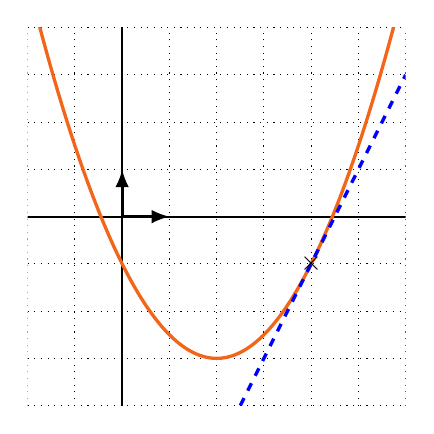
\begin{tikzpicture}[scale=0.6]
\clip (-2,-4) rectangle (6,4);
\draw [thin, dotted] (-2,-4) grid (6,4);
\draw [thick] (-4,0)--(7,0);
\draw [thick] (0,-4) -- (0,5);
\draw [very thick,->,>=latex] (0,0)--(0,1);
\draw [very thick,->,>=latex] (0,0)--(1,0);
\draw [very thick, ocre,domain=-3:6,samples=100] plot (\x,{\x*\x/2-2*\x-1});
\draw [very thick, blue, dashed,domain=-3:6] plot (\x,2*\x-9);
\draw [thick] (4,-1) node {$\times$};
\end{tikzpicture}
\end{center}
\end{minipage}
 \end{example}



\subsection{Variations d'une fonction}

\begin{proposition}Soit $f$ une fonction dérivable sur un intervalle $I$.
\begin{itemize}
\item Si, pour tout $x\in I$, $f'(x) \geqslant 0$, alors $f$ est croissante sur $I$.
\item Si, pour tout $x\in I$, $f'(x) \leqslant 0$, alors $f$ est décroissante sur $I$.
\item Si, pour tout $x\in I$, $f'(x) =0$, alors $f$ est constante sur $I$.
\end{itemize}\end{proposition}

\begin{example}On considère la fonction $f:x\mapsto (x^2-3x+1)\exp(3x+1)$ étudiée précédemment. On a vu que pour tout réel $x$, on a $f'(x)=(3x^2-7x)\exp(3x+1)=x(3x-7)\exp(3x+1)$.

$f'(x)$ étant écrite sous forme factorisée, on peut alors construire le tableau de signes de $f'$ et en déduire les variations de $f$.

\begin{center}
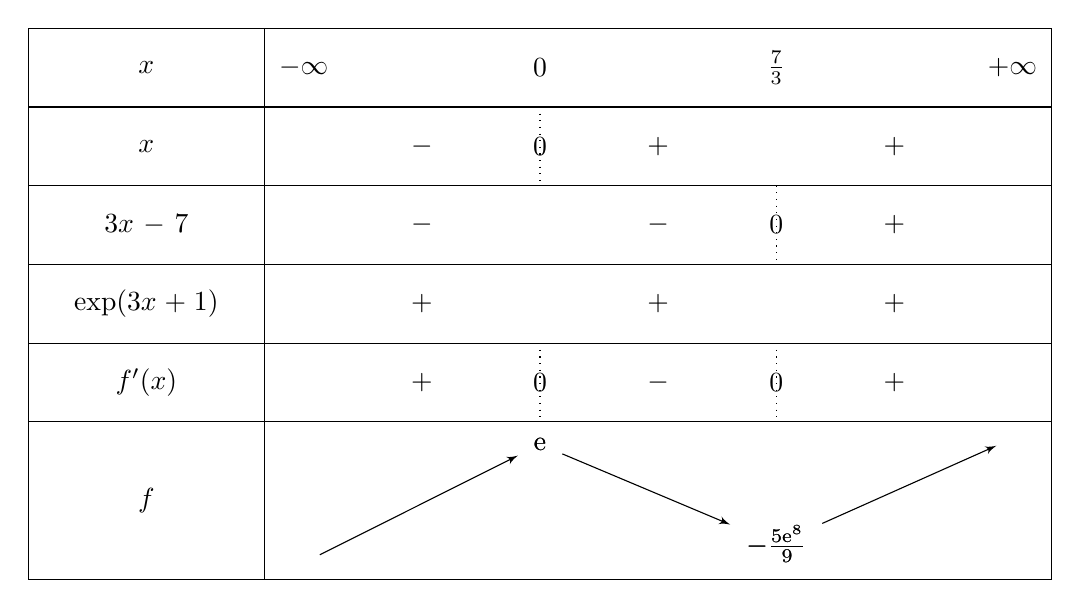
\begin{tikzpicture}[scale=1]
\tikzset{node style/.style = {inner sep = 2pt, outer sep = 2pt}}
   \tkzTabInit[lgt=3]{$x$ / 1 , $x$/1, $3x-7$/1, $\exp(3x+1)$/1, $f'(x)$/1, $f$ / 2}{$-\infty$, $0$, $\frac{7}{3}$,$+\infty$}
   \tkzTabLine{,-,z, +, , +, }
   \tkzTabLine{,-,, -, z, +, }
   \tkzTabLine{,+,, +, , +, }
   \tkzTabLine{,+,z, -, z, +, }
   \tkzTabVar{-/$ $,+/$\e$,-/$-\frac{5\e^8}{9}$,+/$ $}
\end{tikzpicture}\end{center}

\end{example}
\vspace{-0.5cm}


\section{Dérivée seconde}

\begin{definition}[Dérivée seconde] Soit $f$ une fonction dérivable sur un intervalle $I$ telle que sa fonction dérivée $f'$ est également dérivable sur $I$ (on dit également  que $f$ est deux fois dérivable sur $I$).

On appelle fonction \textit{dérivée seconde} de $f$ la fonction dérivée de $f'$. Cette fonction est notée $f''$.
\[ \text{Pour tout } x \in I, \, f''(x)=(f')'(x).\]\end{definition}

\begin{example}Pour tout réel $x$, on pose $f(x)=(2x+1)\e^{3x-2}$. Posons, pour tout réel $x$, $u_1(x)=2x+1$ et $v_1(x)=\e^{3x-2}$.
\begin{itemize}
\item $u_1$ est dérivable sur $\mathbb{R}$ et pour tout réel $x$, $u_1'(x)=2$.
\item $v_1$ est dérivable sur $\mathbb{R}$ et pour tout réel $x$, $v_1'(x)=3\e^{3x-2}$.
\end{itemize}
Ainsi, $f$ est dérivable sur $\mathbb{R}$ et pour tout réel $x$,
\[ f'(x)=u_1'(x) \times v_1(x) + u_1(x) \times v_1'(x) =  2 \times \e^{3x-2} + (2x+1) \times 3\e^{3x-2}=(6x+5)\e^{3x-2}.\]
Posons alors, pour tout réel $x$, $u_2(x)=6x+5$ et $v_2(x)=e^{3x-2}$.
\begin{itemize}
\item $u_2$ est dérivable sur $\mathbb{R}$ et pour tout réel $x$, $u_2'(x)=6$.
\item $v_2$ est dérivable sur $\mathbb{R}$ et pour tout réel $x$, $v_2'(x)=3e^{3x-2}$.
\end{itemize}
Ainsi, $f'$ est dérivable sur $\mathbb{R}$ et pour tout réel $x$,
\[ f''(x)=u_2'(x) \times v_2(x) + u_2(x) \times v_2'(x) =  6 \times e^{3x-2} + (6x+5) \times 3e^{3x-2}=(24x+21)e^{3x-2}.\]
\end{example}



\section{Composition de fonctions}


\begin{definition}[Fonction composée]  Soit $I$ et $J$ deux parties de $\mathbb{R}$.\\ Soit $f$ une fonction définie sur $J$ et $g$ une fonction définie sur $I$ telle que pour tout réel $x$, $g(x) \in J$.

On définit la \textit{fonction composée} de $f$ et $g$ notée $f \circ g$ par 
\[ \text{Pour tout } x \in I, \; f \circ g (x)= f(g(x)).\]\end{definition}
 L'idée derrière la composition de fonctions est simplement d'appliquer successivement plusieurs fonctions.
 \[f \circ g \,:\, x \overset{g}{\longmapsto} g(x) \overset{f}{\longmapsto} f[g(x)]\]

\begin{example} Pour tout réel $x$, on note $f(x)=x^2$ et $g(x)=x+3$. Alors, pour tout réel $x$,
\begin{itemize}
\item $f \circ g (x)= f(g(x))=(g(x))^2=(x+3)^2$.
\item $g \circ f(x)=g(f(x)) = f(x)+3=x^2+3$.
\end{itemize}\end{example}

Attention ! En général, on n'a pas $f \circ g = g \circ f$ ! Ces deux fonctions ne sont d'ailleurs pas forcément définies sur le même ensemble.

\begin{proposition}Soit $I$ et $J$ deux intervalles, $f$ une fonction définie et dérivable sur $J$ et $g$ une fonction définie et dérivable sur $I$ telle que pour tout $x \in I$, $g(x) \in J$. Alors $f \circ g$ est dérivable et pour tout réel $x$ dans $I$,
\[ (f \circ g)' (x)= g'(x) \times (f' \circ g)(x).\]
\vspace{-0.5cm}\end{proposition}



\begin{example}On considère la fonction $f$ définie pour tout réel $x$ par $f(x)=\e^{x^2+3x-2}$. 
Pour tout réel $x$, on pose alors $u(x)=\e^x$ et $v(x)=x^2+3x-2$. Pour tout réel $x$, on a alors  $f(x)= u(v(x)) = u \circ v (x)$.

\begin{itemize}
\item $v$ est dérivable sur $\mathbb{R}$ et pour tout réel $x$, $v'(x)=2x+3$
\item $u$ est dérivable sur $\mathbb{R}$ et pour tout réel $x$, $u'(x)=\e^x$
\end{itemize}
Ainsi, $f$ est dérivable sur $\mathbb{R}$ et pour tout réel $x$, 
\[ f'(x)= v'(x) \times u'(v(x)) = (2x+3)e^{x^2+3x-2}.\]\end{example}
\begin{proposition}[Cas particuliers] Soit $u$ une fonction définie et dérivable sur un intervalle $I$
\begin{itemize}
\item Pour tout entier naturel $n$, $u^n$ est dérivable sur $I$ et $(u^n)'=nu'u^{n-1}$.
\item $e^u$ est dérivable sur $I$ et $(\e^u)'=u' \times \e^u$.
\item Si pour tout réel $x\in I$, $u(x)>0$, alors $\sqrt{u}$ est dérivable sur $I$ et $(\sqrt{u})' = \dfrac{u'}{2\sqrt{u}}$.
\item Si pour tout réel $x$, $u(x) \neq 0$, $\dfrac{1}{u}$ est dérivable sur $I$ et $\left(\dfrac{1}{u}\right)=-\dfrac{u'}{u^2}$.
\end{itemize}\end{proposition}

\begin{example}Pour tout réel $x$, posons $f(x)=(4x+1)^9$.

Pour tout réel $x$, on pose $u(x)=4x+1$. $u$ est dérivable sur $\mathbb{R}$. Or, $f=u^9$.

 Ainsi, $f$ est dérivable sur $\mathbb{R}$ et $f'=9\times u' \times u^8$, c'est-à-dire que pour tout réel $x$, on a
\[ f'(x)= 9 \times 4 \times (4x+1)^{9-1}=36 \times (4x+1)^8.\]\end{example}

\begin{example}Pour tout réel $x$, posons $f(x)=\dfrac{1}{x^2+1}$. 

Pour tout réel $x$, on pose alors $u(x)=x^2+1$. $u$ est dérivable sur $\mathbb{R}$ et ne s'annule pas. Or, $f=\dfrac{1}{u}$.

 Ainsi, $f$ est dérivable sur $\mathbb{R}$ et $f'=-\dfrac{u'}{u^2}$, c'est-à-dire que pour tout $x\in \mathbb{R}$, on a
\[ f'(x)=- \dfrac{2x}{(x^2+1)^2}.\]\end{example}

\begin{example}On considère la fonction $f$ définie pour tout réel $x\in[-2;2]$ par $f(x)=\sqrt{4-x^2}$.

Bien que la fonction $f$ soit définie sur l'intervalle fermé $[-2;2]$, elle n'est en revanche dérivable que sur l'intervalle ouvert $]-2;2[$. Pour tout réel $x\in]-2;2[$, on a
\[f'(x)=\dfrac{-2x}{2\sqrt{4-x^2}}=-\dfrac{x}{\sqrt{4-x^2}}.\]\end{example}




\end{document}